\documentclass[margin=10pt]{standalone}
\usepackage{pgfplots}
\pgfplotsset{compat=1.18}
\usetikzlibrary{arrows.meta, decorations.markings}
\usepackage{amsmath,amssymb}

\begin{document}

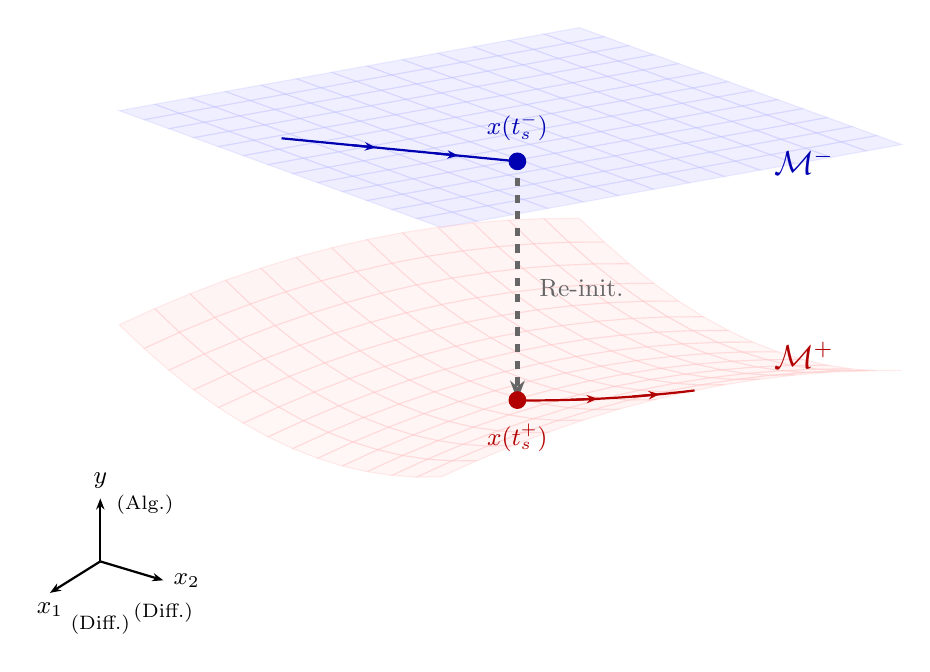
\begin{tikzpicture}
\begin{axis}[
    view={55}{25},
    width=14cm,
    height=12cm,
    axis lines=none,
    clip=false,
    xmin=-2.5, xmax=2.5,
    ymin=-2.5, ymax=2.5,
    zmin=-3.5, zmax=5,
]

% --- Manifold M^- (Pre-switch): gentle plane ---
\addplot3[
    surf,
    opacity=0.3,
    colormap={bluesheet}{color(0)=(blue!12) color(1)=(blue!22)},
    faceted color=blue!25,
    domain=-2:2,
    y domain=-2:2,
    samples=14,
] {0.15*x - 0.1*y + 2.5};

% M^- label on right visible part of surface
\node[blue!70!black, font=\large] at (axis cs: 1.5, 1.5, 2.2) {$\mathcal{M}^-$};

% --- Manifold M^+ (Post-switch): curved saddle ---
\addplot3[
    surf,
    opacity=0.3,
    colormap={redsheet}{color(0)=(red!12) color(1)=(red!22)},
    faceted color=red!25,
    domain=-2:2,
    y domain=-2:2,
    samples=14,
] {0.18*x^2 - 0.12*y^2 - 1.5};

% M^+ label on right visible part of surface
\node[red!70!black, font=\large] at (axis cs: 1.5, 1.5, -1.1) {$\mathcal{M}^+$};

% =============================================
% Switch point at (0.8, -0.5)
% z on M^-: 0.15*0.8 - 0.1*(-0.5) + 2.5 = 2.67
% z on M^+: 0.18*0.64 - 0.12*0.25 - 1.5 = -1.41
% =============================================

% --- Pre-switch trajectory (approaching P^-) ---
\addplot3[
    blue!70!black, thick,
    samples y=0,
    samples=50,
    domain=0:1,
] ({-0.7 + 1.5*x}, {-1.5 + 1.0*x}, {0.15*(-0.7+1.5*x) - 0.1*(-1.5+1.0*x) + 2.5});

% Arrow ticks toward P^-
\draw[-{Stealth[length=4pt, width=3pt]}, blue!70!black, thick]
    (axis cs: -0.25, -1.2, {0.15*(-0.25)-0.1*(-1.2)+2.5})
    -- (axis cs: -0.10, -1.1, {0.15*(-0.10)-0.1*(-1.1)+2.5});
\draw[-{Stealth[length=4pt, width=3pt]}, blue!70!black, thick]
    (axis cs: 0.275, -0.85, {0.15*0.275-0.1*(-0.85)+2.5})
    -- (axis cs: 0.425, -0.75, {0.15*0.425-0.1*(-0.75)+2.5});

% P^- point
\addplot3[only marks, mark=*, mark size=3pt, blue!70!black]
    coordinates {(0.8, -0.5, 2.67)};
\node[blue!70!black, anchor=south, font=\small] at (axis cs: 0.8, -0.5, 2.85) {$x(t_s^-)$};

% --- Re-initialization jump (vertical) ---
\draw[ultra thick, dashed, -{Stealth[length=7pt]}, black!60]
    (axis cs: 0.8, -0.5, 2.67) -- (axis cs: 0.8, -0.5, -1.41);
\node[black!60, anchor=west, font=\small] at (axis cs: 0.95, -0.5, 0.6) {Re-init.};

% --- P^+ point ---
\addplot3[only marks, mark=*, mark size=3pt, red!70!black]
    coordinates {(0.8, -0.5, -1.41)};
\node[red!70!black, anchor=north, font=\small] at (axis cs: 0.8, -0.5, -1.65) {$x(t_s^+)$};

% --- Post-switch trajectory (departing P^+) ---
% Goes from (0.8, -0.5) toward (2.0, 0.2) on M^+
\addplot3[
    red!70!black, thick,
    samples y=0,
    samples=50,
    domain=0:1,
] ({0.8 + 1.2*x}, {-0.5 + 0.7*x}, {0.18*(0.8+1.2*x)^2 - 0.12*(-0.5+0.7*x)^2 - 1.5});

% Arrow ticks away from P^+
\draw[-{Stealth[length=4pt, width=3pt]}, red!70!black, thick]
    (axis cs: 1.16, -0.29, {0.18*1.16^2-0.12*0.29^2-1.5})
    -- (axis cs: 1.34, -0.18, {0.18*1.34^2-0.12*0.18^2-1.5});
\draw[-{Stealth[length=4pt, width=3pt]}, red!70!black, thick]
    (axis cs: 1.58, -0.045, {0.18*1.58^2-0.12*0.045^2-1.5})
    -- (axis cs: 1.76, 0.065, {0.18*1.76^2-0.12*0.065^2-1.5});

\end{axis}

% --- Axis indicator in bottom-left corner ---
\begin{scope}[shift={(1.0, 1.0)}, scale=0.8]
    \draw[-{Stealth[length=4pt]}, thick] (0,0) -- (-0.8, -0.5)
        node[below, font=\small] {$x_1$};
    \draw[-{Stealth[length=4pt]}, thick] (0,0) -- (1.0, -0.3)
        node[right, font=\small] {$x_2$};
    \draw[-{Stealth[length=4pt]}, thick] (0,0) -- (0, 1.0)
        node[above, font=\small] {$y$};
    \node[font=\scriptsize, anchor=north] at (0, -0.7) {(Diff.)};
    \node[font=\scriptsize, anchor=north] at (1.0, -0.5) {(Diff.)};
    \node[font=\scriptsize, anchor=west] at (0.1, 0.9) {(Alg.)};
\end{scope}

\end{tikzpicture}

\end{document}
